\mychapter{Annexes}{cap:annexes}
\lhead{Annexes}

Regroupement des documents servant à l'appui des éléments cités précédemment. Pouvant être de toutes formes (images, blocs de texte, photos...).

% \section{}

% \begin{figure}[H]
%     \centering
%     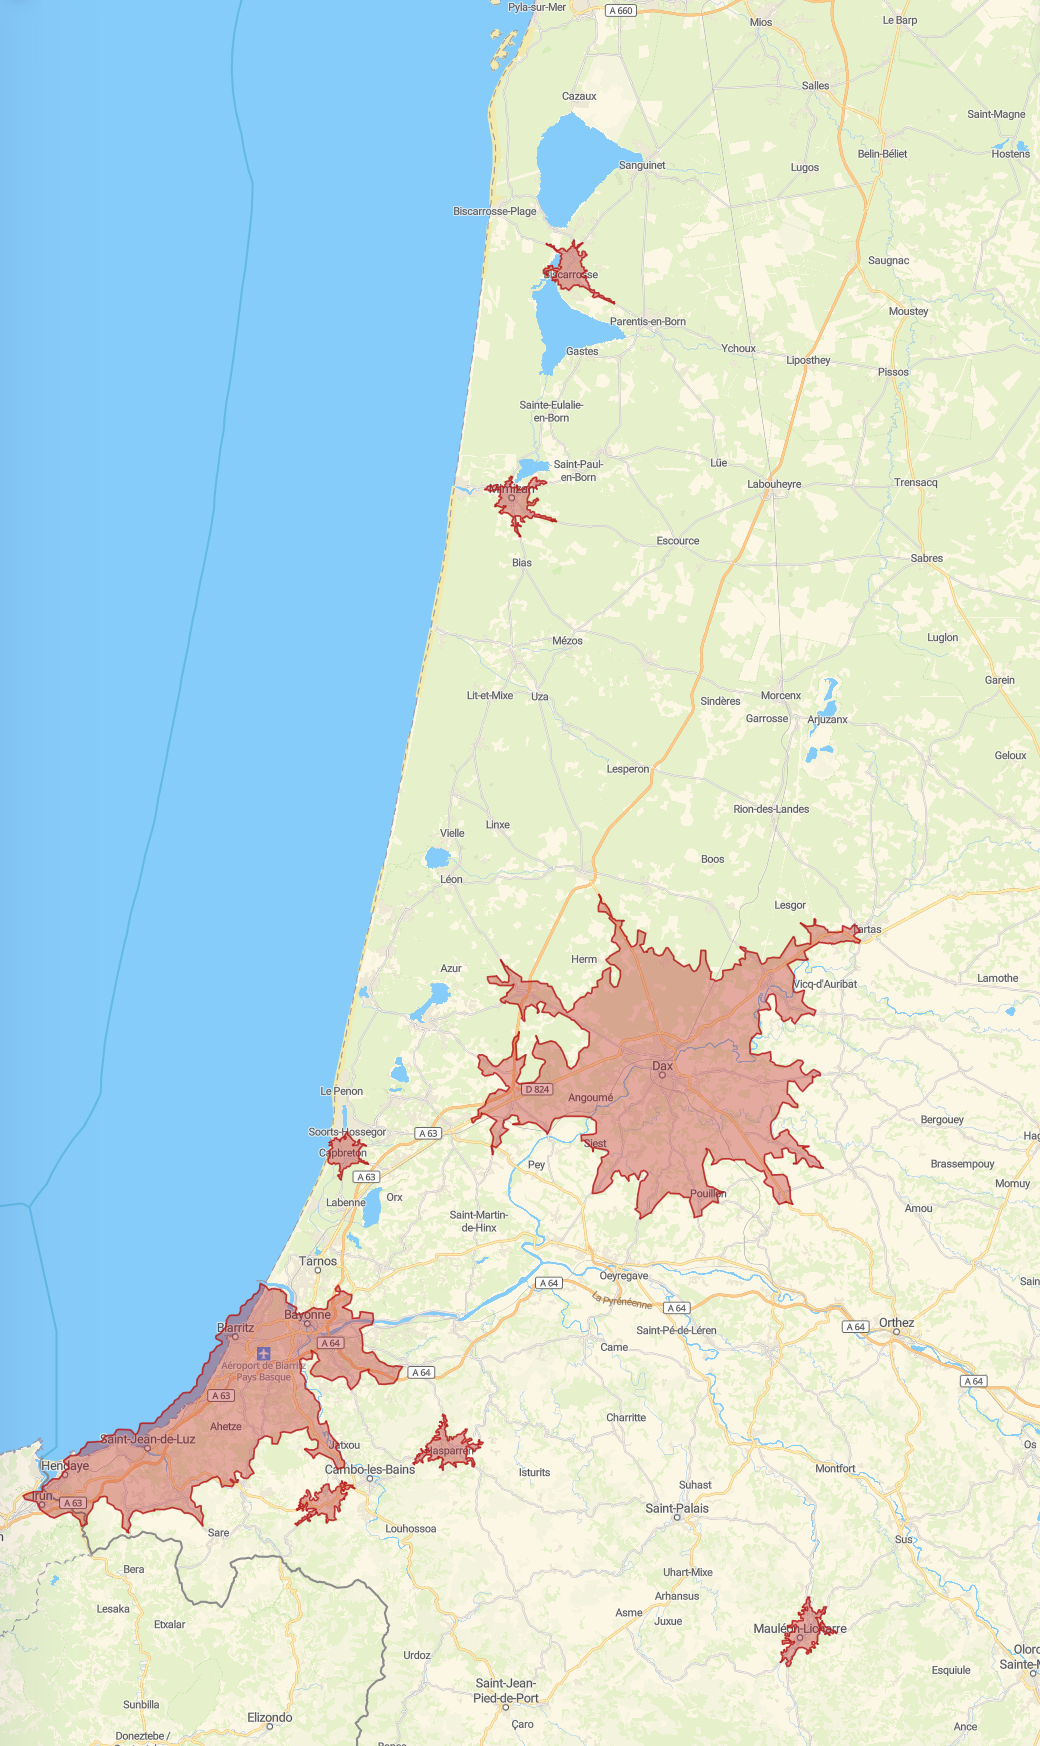
\includegraphics[width=\textwidth - \textwidth / 5]{zone_chalandise_aditu.png}
%     %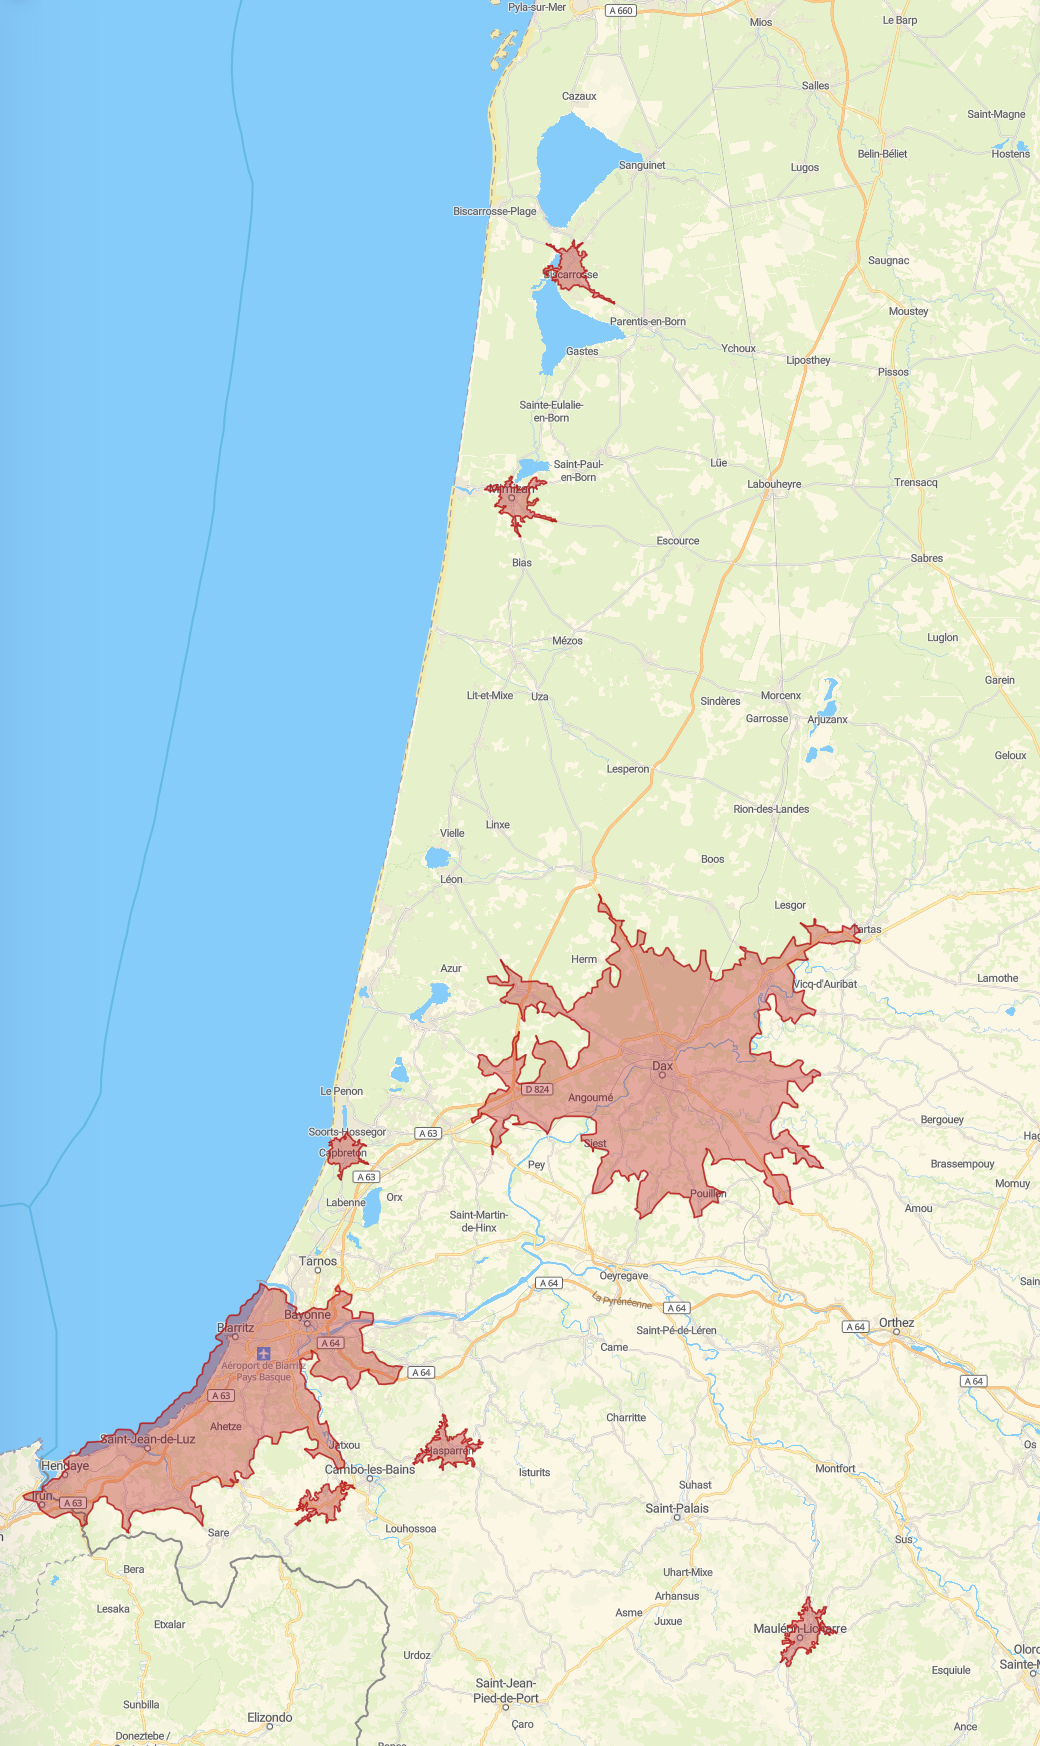
\includegraphics[scale=0.2]{zone_chalandise_aditu.png}
%     \figurename
%     \caption{Visualisation de la zone de chalandise d'ADITU, regroupée autour de ses datacenters à Bidart et à Dax}
%     \label{fig:zone_chalandise}
% \end{figure}

\section{Cahier des charge Ticketing}

% \begin{figure}[H]
%     \centering
%     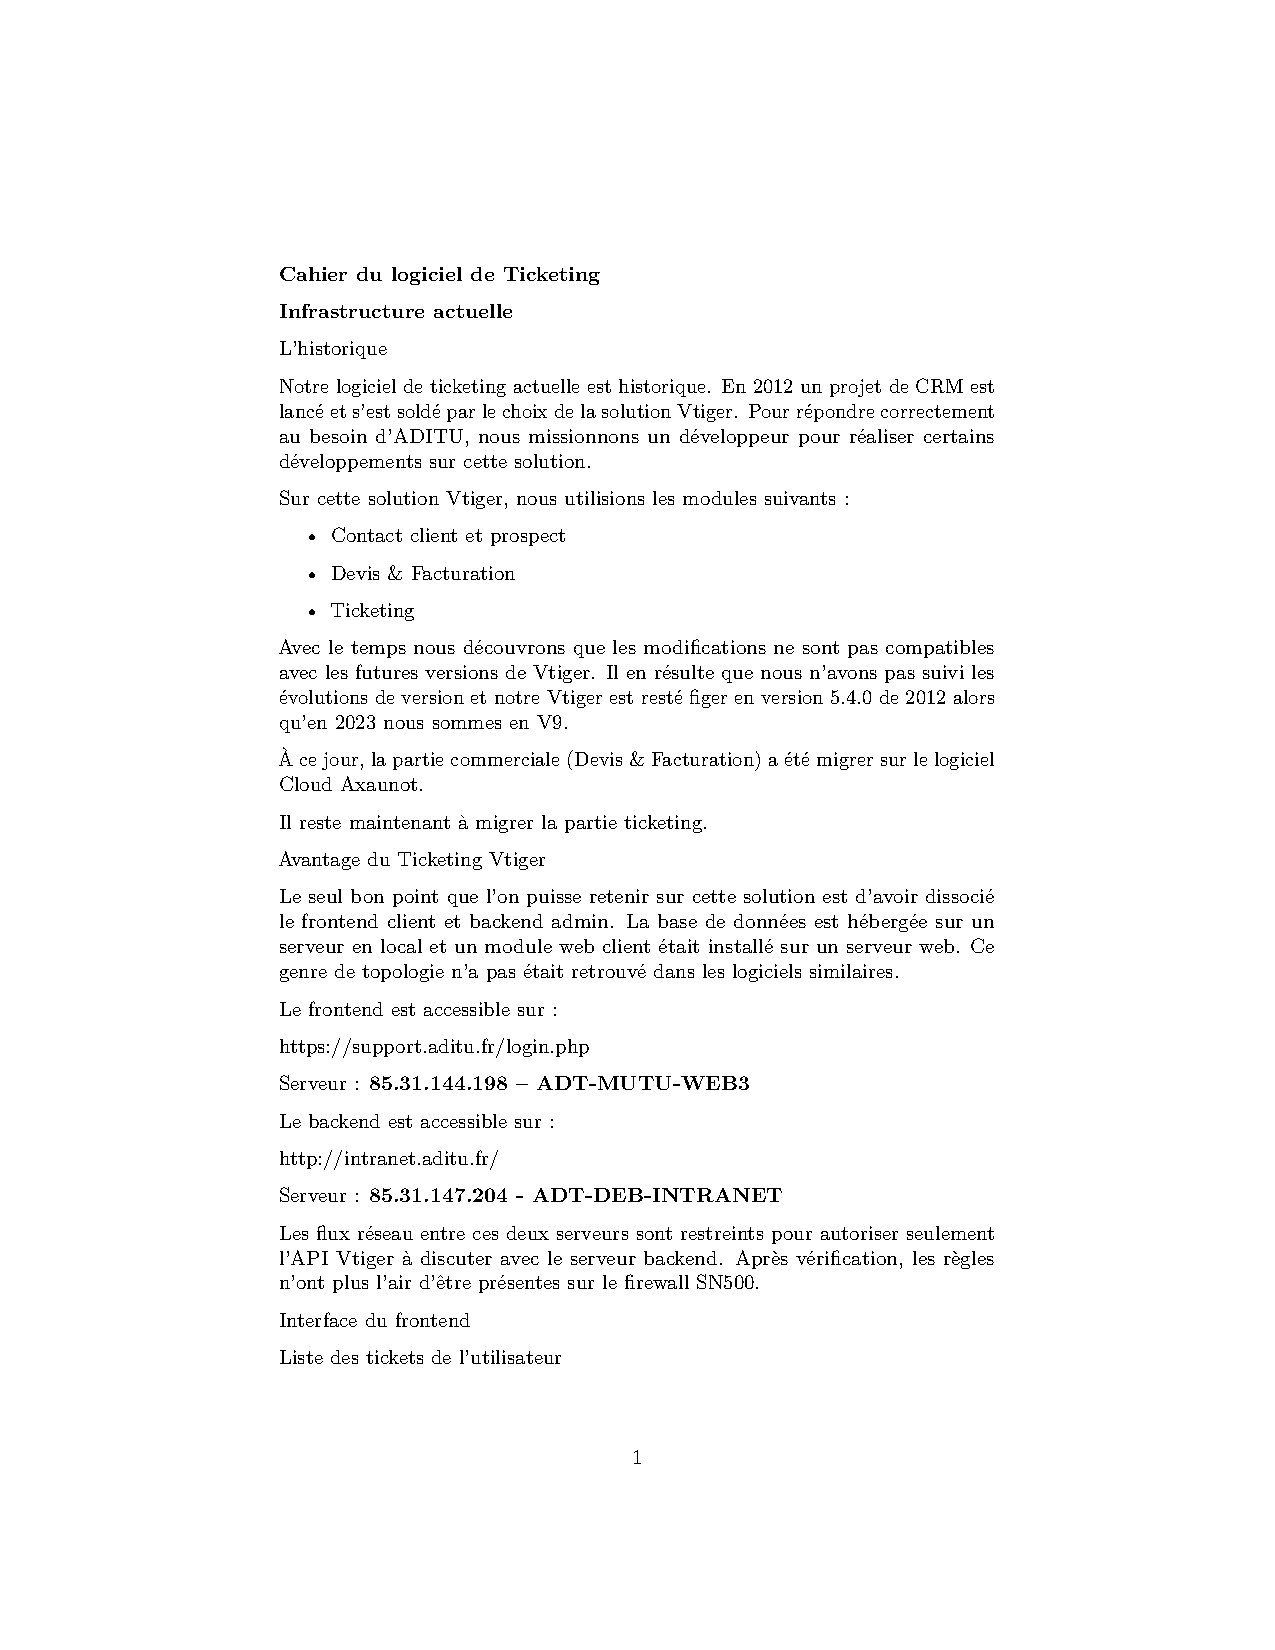
\includegraphics[width=\textwidth - \textwidth / 20]{CDC-Ticketing.pdf}
%     \figurename
%     \caption{Fiche de poste de notre alternance}
%     \label{fig:poste}
% \end{figure}

\textbf{Cahier du logiciel de Ticketing}

\textbf{Infrastructure actuelle}

L'historique

Notre logiciel de ticketing actuelle est historique. En 2012 un projet
de CRM est lancé et s'est soldé par le choix de la solution Vtiger. Pour
répondre correctement au besoin d'ADITU, nous missionnons un développeur
pour réaliser certains développements sur cette solution.

Sur cette solution Vtiger, nous utilisions les modules suivants~:

\begin{itemize}
\item
  Contact client et prospect
\item
  Devis \& Facturation
\item
  Ticketing
\end{itemize}

Avec le temps nous découvrons que les modifications ne sont pas
compatibles avec les futures versions de Vtiger. Il en résulte que nous
n'avons pas suivi les évolutions de version et notre Vtiger est resté
figer en version 5.4.0 de 2012 alors qu'en 2023 nous sommes en V9.

À ce jour, la partie commerciale (Devis \& Facturation) a été migrer sur
le logiciel Cloud Axaunot.

Il reste maintenant à migrer la partie ticketing.

Avantage du Ticketing Vtiger

Le seul bon point que l'on puisse retenir sur cette solution est d'avoir
dissocié le frontend client et backend admin. La base de données est
hébergée sur un serveur en local et un module web client était installé
sur un serveur web. Ce genre de topologie n'a pas était retrouvé dans
les logiciels similaires.

Le frontend est accessible sur~:

\url{https://support.aditu.fr/login.php}

Serveur~: \textbf{85.31.144.198 -- ADT-MUTU-WEB3}

Le backend est accessible sur~:

\url{http://intranet.aditu.fr/}

Serveur~: \textbf{85.31.147.204 - ADT-DEB-INTRANET}

Les flux réseau entre ces deux serveurs sont restreints pour autoriser
seulement l'API Vtiger à discuter avec le serveur backend. Après
vérification, les règles n'ont plus l'air d'être présentes sur le
firewall SN500.

Interface du frontend

Liste des tickets de l'utilisateur

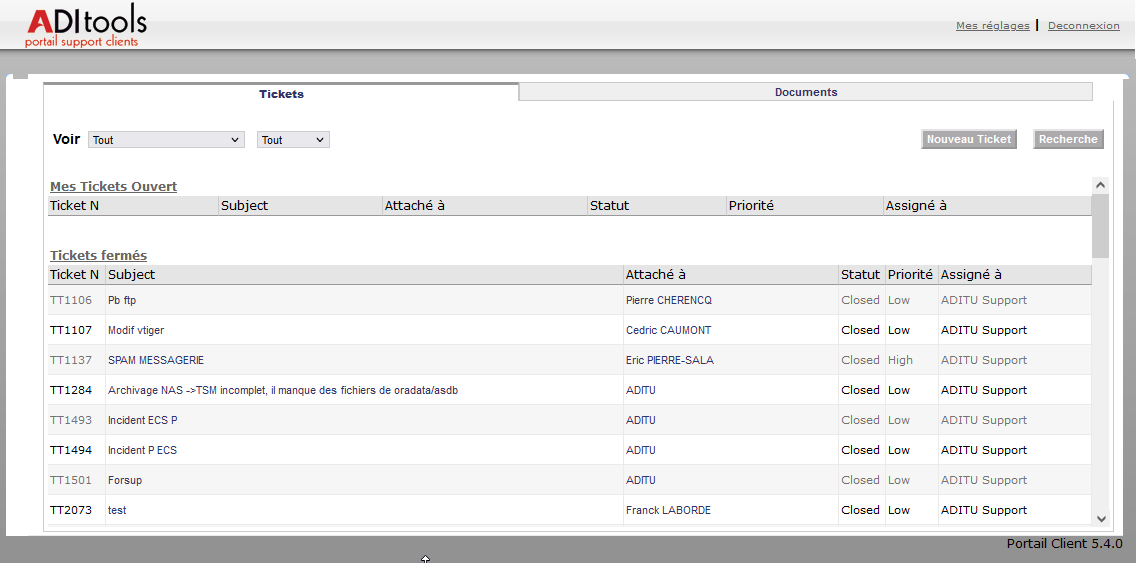
\includegraphics[width=6.3in,height=3.12222in]{image1.png}

Création de tickets

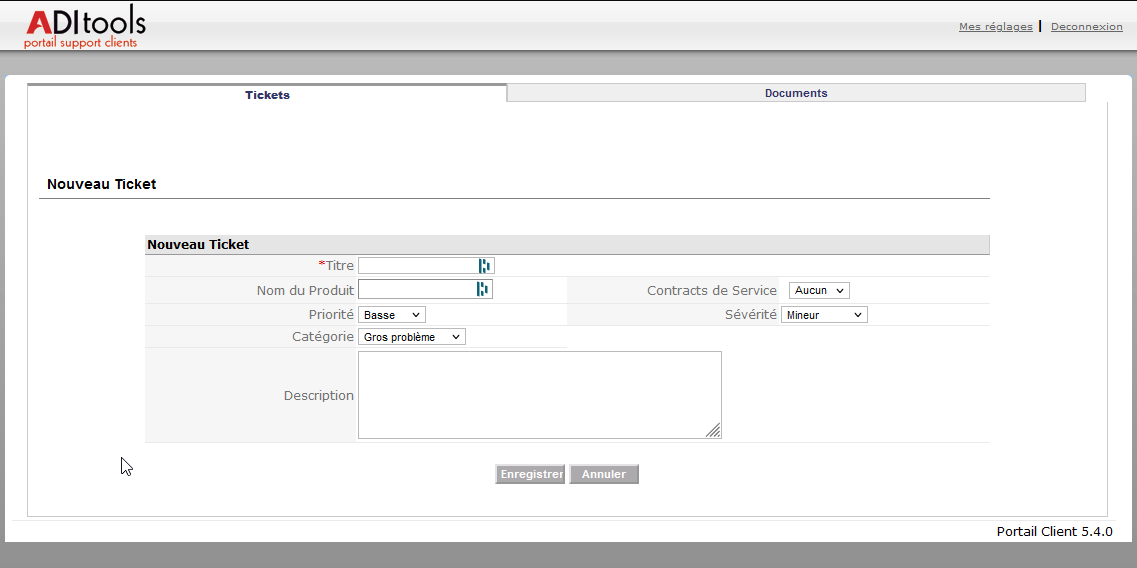
\includegraphics[width=6.3in,height=3.14722in]{image2.png}

On peut constater que l'interface est plutôt minimaliste et
vieillissante. Il manque certaines fonctions qui seront abordées plus
bas.

\textbf{Nouveau logiciel souhaité}

Nous souhaitons migrer vers un nouveau logiciel de ticketing qui puisse
intégrer les fonctionnalités ci-dessous~:

Création d'incidents

\begin{quote}
La gestion des incidents permet de suivre et de résoudre les incidents
signalés par les utilisateurs.
\end{quote}

Création de demandes de changement

\begin{quote}
Gestion des changements permet de planifier, suivre et gérer les
modifications demandées par les utilisateurs.

Exemple~: modification de ports sur le firewall, augmenter une boite aux
lettres, etc.
\end{quote}

Création de tickets automatiquement

\begin{quote}
Cette fonctionnalité permet de planifier des interventions récurrentes
sans les oublier. Exemple~: test de restauration
\end{quote}

Gestion des ressources

\begin{quote}
Pouvoir lié du matériel ou logiciel a un client et faire un suivi des
modifications sur ce cette ressource.

Exemple~: avoir le suivi des modifications comme celui qui est présent
sur la page client du wiki.

Intégrer du matériel lié à un fournisseur et gérer sa garantie. Exemple
NAS ANANDA.

Gérer les renouvellements~: des certificats

Gérer les renouvellements~: des noms de domaines
\end{quote}

Inventaires

\begin{quote}
Lister l'ensemble des machines (connecteur OCS)
\end{quote}

Tableaux de bord et rapports

Avoirs des stats et indicateurs sur ce qui nous prend le plus de temps
dans le support.

Ergonomique

\begin{quote}
Il faut que le logiciel soit intuitif et ergonomique. Que l'utilisateur
ne soit pas rebuté par la complexité d'ouverture d'un ticket.
\end{quote}

Ouverture de ticket via email

Fermeture de ticket automatique après un délai de non-réponse

Personnalisation graphique

\begin{quote}
Nous souhaitons que l'application puisse se personnaliser aux couleurs
de la société et d'y insérer le logo.
\end{quote}

Récupération des données ticketing vtiger

\begin{quote}
Seulement si cette récupération est facile. Ne pas perdre du temps sur
cette récupération.
\end{quote}

Fonctions annexes

Gestion des baies racks du datacenter
